\section{Extra Tests}
\label{app:historical_diagnostics}

This section gives earlier method results, full filter and selector runs,
the first receipt test, parsing details, and extra checks.
Section~\ref{sec:experiments} gives the main results.

\subsection{Earlier Method and Filter Tests}
\label{sec:eval:ablation}

Table~\ref{tab:repair_ablation} compares four saved settings.
The no-completion setting returns the cleaned graph.
Direct LLM uses its own prompt and skips cleanup.
The filter test scores the same proposal before and after checks.
Section~\ref{sec:eval:mechanisms} tests prompt text.
Section~\ref{sec:eval:individual_ablation} tests each filter and selector step.

\begin{table}[t]
\centering
\caption{Four settings on added-defect inputs. Direct LLM uses a different prompt.}
\label{tab:repair_ablation}
\small
\begin{tabular}{l c c c c}
\toprule
Variant & Repair & Over-repair & F1 & Exact \\
\midrule
No LLM completion & 0.3200 & 0.0000 & 0.8472 & 0.0622 \\
Direct LLM (separate prompt) & 0.9244 & 0.0758 & 0.9520 & 0.8267 \\
No constraint gate & 0.9800 & 0.0227 & 0.9895 & 0.9333 \\
\textbf{Diagnosis + Gate} & \textbf{0.9800} & \textbf{0.0167} & \textbf{0.9917} & \textbf{0.9333} \\
\bottomrule
\end{tabular}
\end{table}

Model completion recovers most missing fields.
Diagnosis + Gate reaches 99.17\% F1, compared with 95.20\% for Direct LLM.
Filtering keeps the same repair rate and reduces over-repair by 0.60 points.
It removes eight triples that fail source matching.
All eight differ from the reference.

\subsection{Tests of Filter and Selector Steps}
\label{sec:eval:individual_ablation}

We use 360 Gemma responses from the shared-prompt test and 180 responses
from the new receipt test. We score each under eight filter settings:
all checks, each of five checks removed, duplicate and field-count checks
removed together, and all checks removed. The 540 responses give 4,320
scored outputs. Candidate order stays fixed.
Removing two checks together tests how they affect each other.

Table~\ref{tab:gate_checks} gives full-filter F1 minus each changed-filter
F1. We first average changes across the three prompts for each document,
then across documents. The full filter rejects 28 triples.
Eleven have a wrong document ID and 17 fail source matching.
All 28 differ from the reference. Other checks remove zero extra candidates.
On model-built inputs, source matching adds 0.505 F1 points and the ID check
adds 0.085 points. The 21 adjusted test $p$ values exceed 0.05.
The logs also list correct facts lost when a check is removed.

\begin{table}[t]
\centering
\caption{F1 change from each filter check, in percentage points. Each input group has 60 documents and three prompts. Positive values favour the full filter.}
\label{tab:gate_checks}
\small
\begin{tabular}{lrrr}
\toprule
Removed check(s) & Controlled & Natural & Receipts \\
\midrule
Duplicate & +0.000 & +0.000 & +0.000 \\
Document head & +0.037 & +0.085 & +0.000 \\
Relation type & +0.000 & +0.000 & +0.000 \\
Source support & +0.037 & +0.505 & +0.060 \\
Field count & +0.000 & +0.000 & +0.000 \\
Duplicate + field count & +0.000 & +0.000 & +0.000 \\
All checks & +0.073 & +0.590 & +0.060 \\
\bottomrule
\end{tabular}
\end{table}

\paragraph{Current edit-selector tests.}

We run the v2 selector on saved proposals for 225 added-defect and 225
model-built inputs. Thirteen settings give 5,850 outcomes with the default
absolute prior score. We repeat them with a score relative to equal weights,
giving another 5,850 outcomes. Both runs use \texttt{public-profile-v2}
features and the retrained router. The archive keeps the older v1 runs.

The base setting uses equal weights and keeps the selector on.
Each test changes one named step. The trigger test starts from the
always-on learned-weight setting. Removing a score sets its term to zero
and removes its bounds. Other weights stay the same.
Rule detectors and violation rewards stay active.
Removing rule candidates drops detector actions and direct source-field
additions. The graph profile and saved model proposals stay in use.

\begin{table}[t]

\centering

\caption{V2 selector with the default absolute prior score. Accepted counts are actions or bundles, shown as added-defect / model-built. Each F1 uses 225 documents.}
\label{tab:optimizer_complete}

\small

\begin{tabular}{lrrr}

\toprule

Setting & Controlled F1 & Natural F1 & Accepted \\

\midrule

Always-on uniform & 0.8472 & 0.8833 & 0 / 10 \\

Learned prior, always on & 0.8472 & 0.8799 & 0 / 10 \\

Learned prior and trigger & 0.8472 & 0.8799 & 0 / 10 \\

No prior penalty & 0.8472 & 0.8833 & 0 / 10 \\

No action cost & 0.8930 & 0.8813 & 68 / 13 \\

No density bound & 0.8472 & 0.8833 & 0 / 10 \\

No quality bounds & 0.8472 & 0.8833 & 0 / 10 \\

One iteration & 0.8472 & 0.8833 & 0 / 10 \\

No rule candidates & 0.8472 & 0.8833 & 0 / 9 \\

Rule candidates only & 0.8472 & 0.8799 & 0 / 10 \\

No local score/bounds & 0.8472 & 0.8799 & 0 / 0 \\

No graph score/bound & 0.8472 & 0.8833 & 0 / 10 \\

No source score/bound & 0.8472 & 0.8799 & 0 / 10 \\

\bottomrule

\end{tabular}

\end{table}

The default equal-weight selector reaches 84.72\% F1 on added-defect inputs
and accepts zero edits. Removing edit cost raises F1 to 89.30\% with
68 accepted actions. On model-built inputs, equal weights reach 88.33\% F1.
Learned weights and the learned trigger reach 87.99\%.
Every setting keeps all initially correct reference facts in both groups.
The released files give document scores, trial edits, rejection reasons,
and stop reasons. Holm correction groups the 24 component tests for each
prior score form.

\paragraph{Router training and prior scores.}

The v2 router has an $8\!\rightarrow\!32\!\rightarrow\!16$ network,
one repair output, and three edit-type outputs (884 parameters).
The feature scaler uses 2,098 training rows. Validation and test each have
450 rows grouped by document. Repair and edit-type classification on
added-defect inputs both reach 100\%.
Training labels follow the known added defects.

\begin{table}[t]
\centering
\caption{V2 selector on saved proposals. Relative scores use equal weights as the zero point. Accepted counts are added-defect / model-built.}
\label{tab:math_revision_selector}
\small
\begin{tabular}{lrrr}
\toprule
Prior / offset & Controlled F1 & Natural F1 & Accepted \\
\midrule
Uniform / absolute & 0.8472 & 0.8833 & 0 / 10 \\
Uniform / relative & 0.8472 & 0.8833 & 0 / 10 \\
Learned / absolute & 0.8472 & 0.8799 & 0 / 10 \\
Learned / relative & 0.8929 & 0.8764 & 156 / 51 \\
\bottomrule
\end{tabular}
\end{table}


Table~\ref{tab:math_revision_selector} gives four weight/score settings
from the earlier v2 test. The full runs above include these settings.
With learned weights, the relative score raises added-defect F1 from
84.72\% to 89.29\%. Model-built F1 falls from 87.99\% to 87.64\%.
Both equal-weight settings return the same graphs.
The absolute score remains the default.


\subsection{First Receipt Test}
\label{sec:eval:external_receipts}

We use SROIE receipt text and human field labels \citep{ref_sroie2019}.
A random sample selects 60 of 626 documents from the corrected trainval
mirror (seed 20260922). We join text lines in their stored order.
The model receives this text and four field names: company, date, address,
and total. The scorer reads the field labels.
One receipt has no address label, leaving 239 scored fields.
Every method is scored on these fields.
The model receives all four field names.

Gemma first extracts a graph. Three repair prompts receive this same graph
with the settings in Section~\ref{sec:impl:enhancement}.
We fix samples and settings before calling the model.
The test has 60 extraction calls and 180 repair outputs.
Each repair response is scored before and after filtering.
We also run source copying and rule repair with their original settings.
The main score uses exact triples. A second score ignores case and
whitespace in values.

\begin{table*}[t]
\centering
\caption{First SROIE test on 60 receipts. Exact match uses labelled fields. Normalized F1 ignores case and whitespace in values.}
\label{tab:external_receipts}
\small
\begin{tabular}{lrrrr}
\toprule
Method & Triple F1 & Exact match & Normalized F1 & Facts kept \\
\midrule
Extracted input & 0.7944 & 0.3333 & 0.8153 & 1.0000 \\
Rule Only & 0.7944 & 0.3333 & 0.8153 & 1.0000 \\
Source-field Copy & 0.0000 & 0.0000 & 0.0000 & 0.0000 \\
Base, raw & 0.7944 & 0.3333 & 0.8153 & 1.0000 \\
Base, gate & 0.7915 & 0.3333 & 0.8123 & 0.9944 \\
Diagnostic, raw & 0.7944 & 0.3333 & 0.8153 & 1.0000 \\
Diagnostic, gate & 0.7915 & 0.3333 & 0.8123 & 0.9944 \\
SHACL context, raw & 0.7986 & 0.3333 & 0.8194 & 1.0000 \\
SHACL context, gate & 0.7956 & 0.3333 & 0.8165 & 0.9944 \\
\bottomrule
\end{tabular}
\end{table*}

The input reaches 79.44\% F1. After filtering, base and error-report prompts
both reach 79.15\%. SHACL context reaches 79.56\%.
The error-report minus base difference is $0.00$ points
(95\% CI: $[0.00,0.00]$; paired randomization $p=1.0000$).
Field copying reaches 0.00\% F1 on receipts and 100\% on the named-field
Chinese records.

Of 239 reference values, 220 occur exactly in the source text.
The other 19 differ from the source strings.
Filtering rejects 3 candidates, all matching reference values.
They use the same address in three settings. The source has a double space;
the parser replaces it with a single space in the candidate.
After the run, we apply the same whitespace rule to the source.
All three settings then keep the address.
F1 is 79.44\% for base and error-report prompts and 79.86\% for SHACL.
Exact graph match stays at 33.33\%.
Table~\ref{tab:external_receipts} gives the original-rule scores.

The run has 240 recorded requests, including retries, and 240 parsed outputs.
Mean repair request times are 7.87, 7.92, and 8.05 seconds for base,
error-report, and SHACL prompts. Mean input lengths are 661, 715, and
2276 tokens. Request times include pacing. Extraction and context setup
are counted apart.

\begin{figure}[t]
\centering
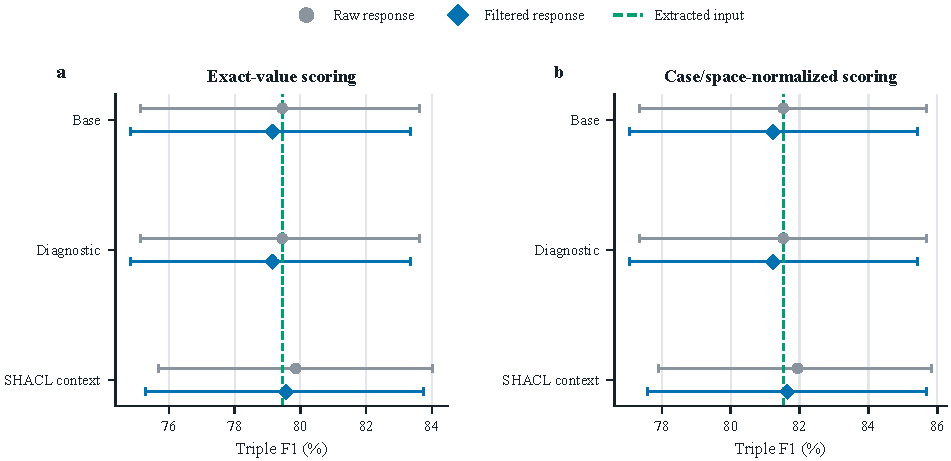
\includegraphics[width=0.98\textwidth]{figure/experiments/external_receipts.pdf}
\caption{First receipt scores. Points show mean F1 and 95\% document-bootstrap CIs. Each raw/gated pair uses one response. The dashed line shows input F1.}
\label{fig:external_receipts}
\end{figure}

\subsection{Receipt Repair and Fresh-Extraction Details}
\label{app:reextraction_diagnostics}

We collect 240 further Gemma responses on the same sixty new-test receipts.
The settings are repair or fresh extraction, with or without the index.
All share source lines, field meanings, document ID, and output limit.
Repair also receives the existing graph. The main score difference is
indexed repair minus indexed fresh extraction after filtering.
All 240 responses have JSON inside Markdown fences.
The fixed strict parser marks them as failures and scores every setting
at zero F1.

After collection, we remove each outer fence and apply the same schema
checks. All 240 responses then parse.
Table~\ref{tab:reextraction_recovery} gives these extra scores.
Indexed repair reaches 83.93\% F1 and indexed fresh extraction reaches
61.05\%. The paired difference is 22.88 points
(95\% CI: 14.84 to 31.35).

\begin{table}[t]
\centering
\caption{Extra scores after collection on sixty receipts. Fence-compatible removes outer Markdown fences. ID-normalized also assigns the known document ID before filtering. Both use the saved responses.}
\label{tab:reextraction_recovery}
\small
\begin{tabular}{lrrr}
\toprule
Method & Fence-compatible F1 & ID-normalized F1 & Wrong-ID graphs \\
\midrule
Fresh extraction & 0.6333 & 0.7256 & 18/60 \\
Indexed extraction & 0.6105 & 0.7486 & 28/60 \\
Repair & 0.7917 & 0.7917 & 0/60 \\
Indexed repair & 0.8393 & 0.8393 & 0/60 \\
\bottomrule
\end{tabular}
\end{table}

Indexed fresh extraction gives the wrong document ID in 28 graphs.
Indexed repair uses the right ID in all sixty.
Assigning the known ID to all four settings raises indexed fresh-extraction
F1 to 74.86\%. Indexed repair leads by 9.07 points
(95\% CI: 5.22 to 13.10). This ID change keeps field values fixed.
The original 22.88-point gap includes both ID and field-value effects.
Initial graph creation is counted apart from these repair calls.

\paragraph{Fields found by the line index.}

We locate the original follow-up's 240 reference fields in the source lines.
Matching keeps case and punctuation and cleans whitespace.
For a value spread over several lines, the index must include all lines of
one occurrence. Of the 240 values, 188 occur in index lines or nearby lines,
36 occur outside them, and 16 differ from the source text.
Among the 188 covered values, Simple returns 163 exactly and Evidence Index
returns 174. Both return 26 of the 36 outside values.
They return zero of the sixteen values that differ from the source.
The index's net gain of eleven exact fields comes from the covered group.

\subsection{Calling Repair after Visible Errors}
\label{app:call_policy}

We test a call rule based on visible ID, relation, duplicate, field-count,
and source-match errors. It selects either the input or the saved repair
output for each document. On the 450-item model-built/clean stream,
it calls repair on 6.22\% of inputs. It misses 63.64\% of graphs with
reference differences. Its F1 is 94.46\%, compared with 95.82\% for
always calling repair. The visible checks miss many missing or wrongly
assigned field values. The main method calls repair on every document.

\paragraph{Useful edits in the earlier selector.}

We use saved proposals and trial graphs from the earlier selector.
These runs came before the shared-feature and candidate-start changes in
Table~\ref{tab:math_revision_selector}. For each document, we try every
subset of model edit bundles and score its graph against the reference.
We apply the saved edits with stopping, cost, and graph-bound checks turned
off. We call the best reference-scored subset the oracle.
This analysis uses model bundles and reference values.

We try 2,144 subsets across 450 inputs.
Table~\ref{tab:selection_bottlenecks} lists the results.
On added-defect inputs, 86 graphs have zero detected violations.
Of these, 72 miss reference fields and 70 have a proposal subset that raises
F1. Among the checked trials, 212 raise reference F1 but have scores of zero
or less. The matching model-built counts are 8 graphs and 1 trial.

\begin{table}[t]
\centering
\caption{Earlier selector results on 225 inputs per group. The oracle uses references to find the best saved subset. One document can have several trials.}
\label{tab:selection_bottlenecks}
\small
\begin{tabular}{lrr}
\toprule
Diagnostic & Controlled & Natural \\
\midrule
Preprocessed graph F1 & 0.8472 & 0.8799 \\
Uniform optimizer F1 & 0.8472 & 0.8833 \\
Fixed-proposal oracle F1 & 0.9964 & 0.9173 \\
Initially no detected violation & 86 & 198 \\
Imperfect among those graphs & 72 & 50 \\
Improvement available among those graphs & 70 & 8 \\
Improving trials with non-positive utility & 212 & 1 \\
\bottomrule
\end{tabular}
\end{table}

Removing edit cost raises F1 on 67 added-defect documents, keeps it the same
on 158, and lowers it on 0. On model-built inputs, it raises F1 on 0,
keeps it the same on 222, and lowers it on 3.
The three graphs with lower F1 already differ from the reference after
cleanup. All 148 exact model-built inputs keep their F1.
The paired added-defect gain is 4.58 points
(95\% document-bootstrap CI: 3.69--5.54).
The same cost change has different effects on the two input groups.


\subsection{Time and Memory for Graph Checks}
\label{sec:eval:scale}

We time the report in Eq.~(\ref{eq:diagnostic_context}) on separate document
batches with 1K--50K triples. A full pass checks every document.
A local update checks one changed document.
Full times are medians of seven runs. Local times are medians of 200 runs.
Table~\ref{tab:diagnostic_scaling} gives the values.
Memory measures the peak new Python memory for building the batch.
Source text and schema objects are shared. Model-call times are recorded apart.

\begin{figure}[t]
\centering
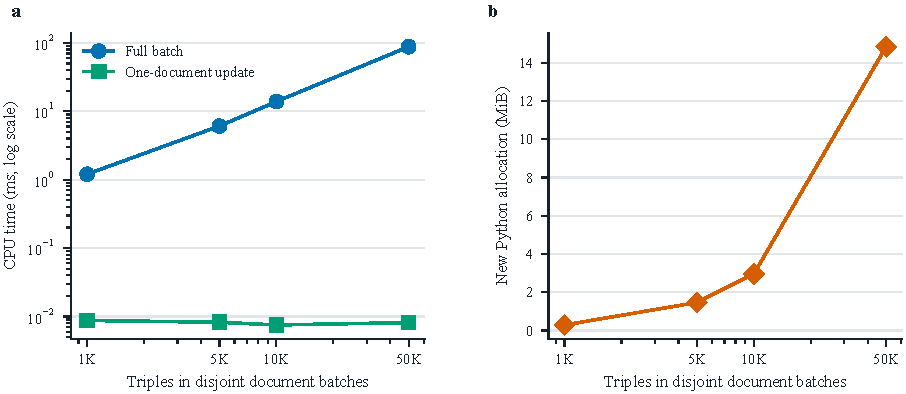
\includegraphics[width=0.98\textwidth]{figure/experiments/diagnostic_scaling.pdf}
\caption{Time and memory for reports on separate document batches. Local updates check one changed document. Memory measures new batch storage with shared source text.}
\label{fig:diagnostic_scaling}
\end{figure}

\subsection{Extra Quality and Extraction Checks}
\label{sec:eval:external_benchmark}

A Gemma judge scores 180 source--triple pairs with method names hidden.
Its source score has Pearson $r=0.794$ and Spearman $\rho=0.807$ with
exact reference validity (both $p<2.4\times10^{-40}$).
A fixed 50-item sample has the same mean, 0.96, in five further runs.

We compare our extractor with Neo4j Labs' \texttt{LLMGraphTransformer}
core on 45 balanced TNEWS documents \citep{ref_neo4j_llm_graph_builder}.
Category accuracy is 0.556 for our field-based extractor and 0.533 for
Graph Builder. The paired test gives $p=1.00$.

\subsection{Request Costs and Check Times}
\begin{table*}[t]
\centering
\caption{Request costs. Mean times include retries and pacing. Source setup and queue time are counted apart.}
\label{tab:matched_cost}
\small
\resizebox{\textwidth}{!}{%
\begin{tabular}{llrrrr}
\toprule
Input & Context & Calls & Input tokens & Output tokens & Wall (s) \\
\midrule
Controlled & Base & 1.00 & 947 & 517 & 8.58 \\
Controlled & Diagnostic & 1.00 & 1017 & 512 & 8.61 \\
Controlled & SHACL & 1.00 & 3080 & 513 & 8.45 \\
Natural & Base & 1.00 & 832 & 458 & 7.51 \\
Natural & Diagnostic & 1.00 & 901 & 462 & 7.90 \\
Natural & SHACL & 1.00 & 2822 & 455 & 8.16 \\
\bottomrule
\end{tabular}%
}
\end{table*}
\begin{table*}[t]
\centering
\caption{Time and memory for graph reports. Memory counts peak new batch storage in MiB. Source texts are shared.}
\label{tab:diagnostic_scaling}
\small
\resizebox{\textwidth}{!}{%
\begin{tabular}{rrrrr}
\toprule
Triples & Documents & Full (ms) & Local (ms) & Memory (MiB) \\
\midrule
1,000 & 143 & 1.20 & 0.009 & 0.29 \\
5,000 & 716 & 6.08 & 0.008 & 1.47 \\
10,000 & 1,434 & 13.90 & 0.008 & 2.96 \\
50,000 & 7,173 & 88.10 & 0.008 & 14.84 \\
\bottomrule
\end{tabular}%
}
\end{table*}

